% UGA Dissertation Template
% Changes to official template by Kyle Krafka (December 2015)

\documentclass[12pt,notitlepage]{report}  % The notitlepage option prevents \maketitle from resetting page numbering, below.
\usepackage{kyle}
\usepackage{fullpage}
\usepackage{setspace}\doublespacing
\textfloatsep 0.75in
\usepackage[nottoc]{tocbibind}  % Added nottoc option to remove "Contents"
\usepackage{graphicx}
\usepackage{subcaption}
\usepackage{wrapfig}
\usepackage[hidelinks]{hyperref}  % Allows you to click on references in the PDF.
\usepackage[square]{natbib}  % Use name/year for citations rather than numbers.
\usepackage{amsmath}
\usepackage{MinionPro}  % Serif font.
\usepackage{MyriadPro}  % Sans-serif font.
\usepackage{pgfornament}  % For the ornament, used on the dedication page.
% \usepackage{longtable}
% This makes for a larger left margin so that when you bind your dissertation,
% the text stays away from the binding. From what I have seen, people typically
% have it bound single-sided (i.e., the back of each page is blank), but if you
% want it double-sided, use the "twoside" option right before or after the
% "bindingoffset" option here (with a comma). The choice of 6 mm was mostly
% arbitrary, but The Graduate School recommended anywhere from 0 to 0.5 inches
% of binding offset on top of the 1 in left margin.
\usepackage[bindingoffset=6mm]{geometry}
\usepackage[toc]{appendix}  % Allows for an appendix, which should appear in the table of contents.
\usepackage[english]{babel}
\usepackage{lipsum}  % Generates dummy text

% Title
\newcommand{\dissertationtitle}{My Awesome Complex\\and Totally-Smart Dissertation Title}
\newcommand{\whoami}{Kyle John Krafka}

\setcounter{tocdepth}{1}

\begin{document}

% Make the official abstract page
\newpage
\thispagestyle{empty}
\vspace*{18pt}
\begin{center}
\textsc{\large{\dissertationtitle}}\\[18pt]  % A little larger than the original template
by\\[18pt]
\textsc{\whoami}\\[12pt]
(Under the Direction of Bobby Joe)\\[12pt]
\textsc{Abstract}
\end{center}
Here is my abstract. Here is my abstract. Here is my abstract. Here is my
abstract. Here is my abstract. Here is my abstract. Here is my abstract. Here is
my abstract. Here is my abstract. Here is my abstract. Here is my abstract.
\thispagestyle{empty}

\begin{list}{\textsc{Index words:\hfill}}{\labelwidth 1.2in\leftmargin 1.4in\labelsep 0.2in}
\item 
\begin{flushleft}\singlespacing
Cool stuff,
Deep learning,
Big data,
Crowdsourcing,
Computer vision,
Computer science
\end{flushleft}
\end{list}

% Make the official title page
\newpage
\pagenumbering{roman}
\thispagestyle{empty}
\vspace*{18pt}
\begin{center}
\textsc{\large{\dissertationtitle}}\\[18pt]
by\\[18pt]
\textsc{\whoami}\\[12pt]
B.S., University of Georgia, 2010\\
\vfill
A Dissertation Submitted to the Graduate Faculty \\
of The University of Georgia in Partial Fulfillment \\
of the \\
Requirements for the Degree \\[10pt]
\textsc{Doctor of Philosophy}\\[36pt]
\textsc{Athens, Georgia}\\[18pt]
2015
\end{center}

% Make the copyright page
\newpage
\thispagestyle{empty}
\vspace*{5.5in}
\begin{center}
\copyright 2015 \\
\whoami \\
All Rights Reserved
\end{center}

% Make the approval page
\newpage
\thispagestyle{empty}
\vspace*{18pt}
\begin{center}
\textsc{\large{\dissertationtitle}}\\[18pt]
by\\[18pt]
\textsc{\whoami}
\end{center}
\vfill
\begin{flushleft}\singlespacing
\hskip 200pt {Approved:}\\
\vskip 12pt

% If you have two major professors, change "Professor" to "Professors."
\hspace*{200pt}\makebox[100pt][l]{Major Professor:}Bobby Joe\\
\vskip 12pt
% Committee (use as many lines as needed)
\hspace*{200pt}\makebox[100pt][l]{Committee:       }Jane Doe\\
\hspace*{200pt}\makebox[100pt][l]{~                }Billy Bob\\
% Approval words
\vfill
Electronic Version Approved:\\[12pt]
Suzanne Barbour\\
Dean of the Graduate School\\
The University of Georgia\\
December 2015
\end{flushleft}

% This title page is not in the style manual, but it is in the original template.
\title{\textbf{\dissertationtitle}}
\author{\whoami}
\date{December 2015}
\maketitle
\thispagestyle{empty}

\newpage
\vspace*{1.5in}
\begin{center}
\emph{For Mom and Dad}\\
\vspace{1cm}
\pgfornament[width = 4cm,
             color = black]{88}  % Feel free to download the pgfornament manual to choose your own ornament.
\end{center}

\chapter*{Acknowledgments}
% chapter* removes chapter number, but also removes from TOC, so we add it back
\addcontentsline{toc}{chapter}{Acknowledgments}

All of your acknowledgments should go here.
\lipsum

\tableofcontents
\listoffigures  % If any.
\listoftables % If any.
\clearpage
\pagenumbering{arabic}

% Chapters. Organize and name as you wish, as long as these refer to files that exist.
%%%%%%%%%%%%%%%%
% INTRODUCTION %
%%%%%%%%%%%%%%%%
\chapter{Introduction}

% TODO: Include a second citation. Include \eg \ie examples. Include references. Include em dash.
Here is the introduction. My dissertation introduces \emph{widgets}. If I wish
to cite someone, I could refer to them in text as in \citet{zongker2006chicken},
or parenthetically \citep{zongker2006chicken}. I can also cite just the
year \citeyearpar{zongker2006chicken} or mention the author,
\citeauthor{zongker2006chicken}.

I can use macros (\eg, the ones defined in \texttt{kyle.sty}). \Ie, just like
I am doing in the source.

\begin{quote}
This dissertation template is handy. I like it and use it every time I write a
dissertation.\\
\hspace*{\fill} --- Abraham Lincoln \citeyearpar{zongker2006chicken}
\end{quote}


\section{Stuff}
\label{sec:stuff}

Here is a section on stuff.

\subsection{Artificial Neural Networks}
\label{sec:neuralnet}

See Figure \ref{fig:neuralnet} for a neural network.

\begin{figure}[th]
	\begin{center}
	   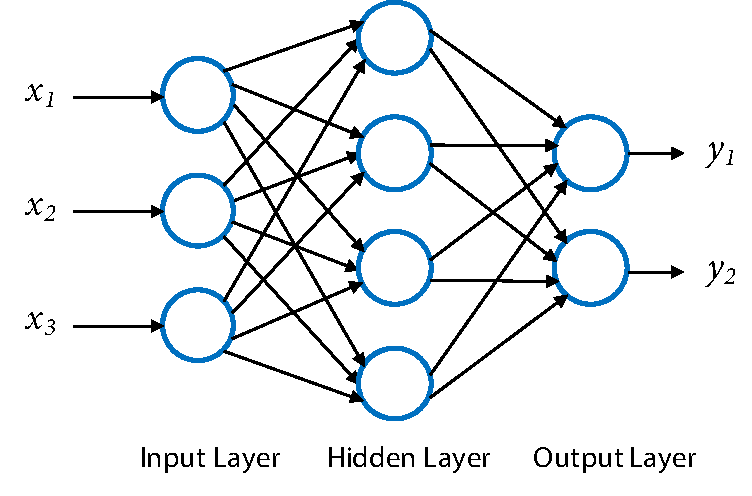
\includegraphics[width=0.8\linewidth]{figures/neuralnet}
	\end{center}
	\caption[An example neural network with two final outputs]
		{An example neural network with two final outputs. Notice how each
		neuron in one layer connects to each neuron in the following layer. This
		is called \emph{fully connected}.}
	\label{fig:neuralnet}
\end{figure}

Cool.
%%%%%%%%%%%%%%%%
% RELATED WORK %
%%%%%%%%%%%%%%%%
% Or ``Review of the Literature''
\chapter{Related Work}
\label{ch:related_work}

Stuff.
%%%%%%%%%%%%%%%
% METHODOLOGY %
%%%%%%%%%%%%%%%
\chapter{Methodology}
\label{ch:methodology}

\lipsum
%%%%%%%%%%%%%%%
% EXPERIMENTS %
%%%%%%%%%%%%%%%
\chapter{Experiments}
\label{ch:experiments}

Check out Table \ref{tbl:calibration}. You might consider using
\texttt{longtable} or \texttt{tabu} for your tables instead.

\begin{table}
  \centering
  \small
  \begin{tabular}{crr}
    \hline
    Count & $x$ Error & $y$ Error\\\hline\hline
    4 & 2.30 & 2.30\\\hline
    5 & 2.10 & 1.97\\\hline
    9 & 1.92 & 1.72\\\hline
    13 & 1.82 & 1.64\\\hline
  \end{tabular}
  \caption[Effect of count on error]
    {Effect of count on error using our model. The error reduces as the count
    increases.}
  \label{tbl:calibration}
\end{table}

\lipsum
%%%%%%%%%%%%%%
% CONCLUSION %
%%%%%%%%%%%%%%

\chapter{Conclusion}
\label{ch:conclusion}

\lipsum

\begin{appendices}
	\chapter{Extended Results}

% For data tables, check out the longtable package.

\lipsum
\end{appendices}

\newpage
\bibliographystyle{plainnat}
\bibliography{dissertation}

\end{document}
